\documentclass[12pt,letterpaper,twocolumn,openany,nodeprecatedcode,bg=none]{dndbook}
\usepackage[english]{babel}
\usepackage[utf8]{inputenc}
\usepackage{longtable,booktabs,array}
\usepackage{calc}
\usepackage{etoolbox}
\usepackage{caption}
\AtBeginEnvironment{longtable}{\small}

% Fix for Pandoc 3.1.7+ image handling
\providecommand{\pandocbounded}[1]{#1}

% Pandoc's compact list helper
\providecommand{\tightlist}{%
  \setlength{\itemsep}{0pt}\setlength{\parskip}{0pt}}

% Remove "Figure N:" prefix from captions
\captionsetup{labelformat=empty}

% Remove section numbering
\setcounter{secnumdepth}{0}

\begin{document}

\title{Evoker}
\author{Class Handbook}
\date{}
\maketitle

\onecolumn

\emph{Your trusty class handbook for the Old Scrolls roleplaying game.}

\clearpage

\begin{figure}
\centering
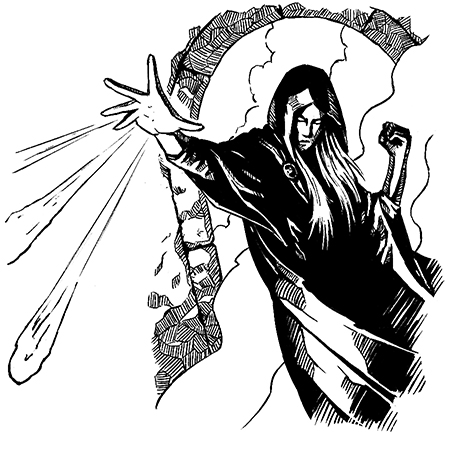
\includegraphics[width=1\linewidth,height=\textheight,keepaspectratio]{magicMissile.jpg}
\caption{\emph{A pyromancer blasts away their foes}}
\end{figure}

\clearpage

\section{Evoker}\label{evoker}

As an evoker, you have learned how to harness one of the three core
magical energies, fire, frost, and shock. Rather than take a generalist
approach to magic where you learn specific spells, you focus instead on
specializing and wielding your elemental energy to the fullest effect.

\subsection{Core Evoker Traits}\label{core-evoker-traits}

\begin{longtable}[]{@{}
  >{\raggedright\arraybackslash}p{(\linewidth - 2\tabcolsep) * \real{0.2542}}
  >{\raggedright\arraybackslash}p{(\linewidth - 2\tabcolsep) * \real{0.7458}}@{}}
\toprule\noalign{}
\begin{minipage}[b]{\linewidth}\raggedright
\textbf{Primary Ability}
\end{minipage} & \begin{minipage}[b]{\linewidth}\raggedright
Wisdom
\end{minipage} \\
\midrule\noalign{}
\endhead
\bottomrule\noalign{}
\endlastfoot
\textbf{Hit Points} & 8 at 1st level, 6 per level gained after 1st \\
\textbf{Saving Throw Proficiencies} & Wisdom, Charisma \\
\textbf{Skill Proficiencies} & Choose any 2 skills. If you choose a
skill you already have, you gain expertise with it. \\
\textbf{Weapon Proficiencies} & Choose 1: Blade, Blunt, Bow, Mechanical,
Polearm, and Shield \\
\textbf{Starting Equipment} & Padded Jacket, Sabre, Dagger, Grimoire \\
\end{longtable}

\subsection{Evoker Features}\label{evoker-features}

\begin{longtable}[]{@{}
  >{\raggedright\arraybackslash}p{(\linewidth - 8\tabcolsep) * \real{0.0641}}
  >{\raggedright\arraybackslash}p{(\linewidth - 8\tabcolsep) * \real{0.1410}}
  >{\raggedright\arraybackslash}p{(\linewidth - 8\tabcolsep) * \real{0.1410}}
  >{\raggedright\arraybackslash}p{(\linewidth - 8\tabcolsep) * \real{0.0641}}
  >{\raggedright\arraybackslash}p{(\linewidth - 8\tabcolsep) * \real{0.5897}}@{}}
\toprule\noalign{}
\begin{minipage}[b]{\linewidth}\raggedright
Level
\end{minipage} & \begin{minipage}[b]{\linewidth}\raggedright
Proficiency
\end{minipage} & \begin{minipage}[b]{\linewidth}\raggedright
Mana Points
\end{minipage} & \begin{minipage}[b]{\linewidth}\raggedright
Power
\end{minipage} & \begin{minipage}[b]{\linewidth}\raggedright
Class Features
\end{minipage} \\
\midrule\noalign{}
\endhead
\bottomrule\noalign{}
\endlastfoot
1 & +2 & 2 & 1 & Evocation, Elemental Specialty \\
2 & +2 & 3 & 1 & Evocation Technique \\
3 & +2 & 6 & 2 & Specialty Power, Unfettered Arcana \\
4 & +2 & 6 & 2 & Ability Score Improvement, Evocation Technique \\
5 & +3 & 12 & 3 & Specialty Power \\
6 & +3 & 12 & 3 & Evocation Technique \\
7 & +3 & 16 & 4 & Specialty Power \\
8 & +3 & 20 & 4 & Ability Score Improvement, Evocation Technique \\
9 & +4 & 25 & 5 & Specialty Power \\
10 & +4 & 25 & 5 & Evoker's Mastery, Evocation Technique \\
\end{longtable}

\twocolumn

\subsection{Evoker Features}\label{evoker-features-1}

As an evoker, you gain the following class features when you reach the
specified levels. These features are listed on the Evoker Features
table.

\subsection{Level 1: Evocation}\label{level-1-evocation}

You have learned to harness the elemental powers of magic.

\textbf{Spellcasting Ability.} Wisdom is the spellcasting ability for
evoker features. If you make an attack roll with an evoker spell or
feature, your bonus is your spellcasting modifier plus your proficiency
bonus. The saving throw DC of your spells is 8 + your spellcasting
modifier + your proficiency bonus.

\textbf{Spell Power.} When you use an evoker feature, its effects might
be determined by your power. Many features have effects that scale, such
as damage, based on your power.

\textbf{Mana Points.} Your magic is powered by mana. You gain mana
points as indicated in the Evoker Features table. You can spend a number
of points per turn up to your power.

You regain up to a number of mana points equal to your power when you
finish a short rest, and all expended mana points when you finish a long
rest.

\textbf{Arcane Bolt.} As a magic attack action, you can make a ranged
attack against a target within 120 feet. On a hit, this attack does 1d10
+ your spellcasting modifier damage. The damage increases to 2d10 if
your power is 3 or greater and 3d10 if your power is 5 or greater. The
damage type is either fire, cold, lightning, or thunder depending on
your elemental specialty.

Before rolling your attack you can expend a mana point to increase the
damage by 1d10 per point spent, and the target takes half damage on a
miss.

\subsection{Level 1: Elemental
Specialty}\label{level-1-elemental-specialty}

Every evoker has a an especially strong connection with one flavor of
the raw magical elements, fire, frost, and shock. Choose one of the
elemental specialties provided below.

\subsection{Level 2: Evocation
Technique}\label{level-2-evocation-technique}

As you gain more elemental power, you exert more control over your magic
and begin to shape it into more specific effects. You gain an Evocation
feat of your choice.

Whenever you gain an evoker level, you can replace the feat you chose
with a different Evocation feat.

\subsection{Level 3: Specialty Power}\label{level-3-specialty-power}

You gain access to another power from your Elemental Specialty.

\subsection{Level 3: Unfettered Arcana}\label{level-3-unfettered-arcana}

You gain the Unfettered Arcana benefit listed for your Elemental
Specialty.

\subsection{Level 4: Ability Score
Improvement}\label{level-4-ability-score-improvement}

You gain a +1 bonus to two abilities of your choice.

\subsection{Level 4: Evocation
Technique}\label{level-4-evocation-technique}

As you gain more elemental power, you exert more control over your magic
and begin to shape it into more specific effects. You gain an Evocation
feat of your choice.

\subsection{Level 5: Specialty Power}\label{level-5-specialty-power}

You gain access to another power from your Elemental Specialty.

\subsection{Level 6: Evocation
Technique}\label{level-6-evocation-technique}

As you gain more elemental power, you exert more control over your magic
and begin to shape it into more specific effects. You gain an Evocation
feat of your choice.

\subsection{Level 7: Specialty Power}\label{level-7-specialty-power}

You gain access to another power from your Elemental Specialty.

\subsection{Level 8: Ability Score
Improvement}\label{level-8-ability-score-improvement}

You gain a +1 bonus to two abilities of your choice.

\subsection{Level 8: Evocation
Technique}\label{level-8-evocation-technique}

As you gain more elemental power, you exert more control over your magic
and begin to shape it into more specific effects. You gain an Evocation
feat of your choice.

\subsection{Level 9: Specialty Power}\label{level-9-specialty-power}

You gain access to another power from your Elemental Specialty.

\subsection{Level 10: Evoker's Mastery}\label{level-10-evokers-mastery}

Work with your DM to create a custom spell that reflects your
character's uniqueness!

\subsection{Level 10: Evocation
Technique}\label{level-10-evocation-technique}

As you gain more elemental power, you exert more control over your magic
and begin to shape it into more specific effects. You gain an Evocation
feat of your choice.

\clearpage

\section{Elemental Specialties}\label{elemental-specialties}

Here are the elemental specialties to choose from. Each specialty gives
you a set of core benefits, along with expanded benefits as your level
increases.

\subsection{Pyromancy}\label{pyromancy}

You are trained in the power of fire, a destructive force that burns
away your enemies. Fire is impossible to fully control. When you use
your magic, you merely direct the power you tap into and are sometimes
as surprised at the effects as others.

\subsubsection{Burning Flames}\label{burning-flames}

When rolling fire damage, if you roll the maximum possible result on a
die you may roll an additional die of that type as additional fire
damage. This benefit applies to the additional die you roll.

\subsubsection{Flickering Flame}\label{flickering-flame}

As a magic action, you can cause fire to erupt from one of your hands.
This fire sheds bright light for 20 feet and dim light for an additional
20 feet. As an action, you can touch a flammable object in melee range
and cause it to ignite. You can choose to douse your hand on your turn
without using an action.

\subsubsection{Gout of Flame}\label{gout-of-flame}

As a magic attack action, you can make a ranged attack against up to
three targets within 30 feet. On a hit, this attack does 1d6 + your
spellcasting modifier fire damage. The damage increases to 2d6 if your
power is 3 or greater and 3d6 if your power is 5 or greater.

You can expend mana points to increase the attacks' damage by 2d6 per
point spent, and a target takes half damage on a miss. Spend these
points before rolling your attacks.

\subsubsection{Power 2: Cinder Cloud}\label{power-2-cinder-cloud}

If your power is 2 or greater, you can use a magic action and expend 1
or more mana points to cause a great gout of smoke and cinders to erupt
from your hands. Choose a point within range. The area within a 20-foot
radius of that point fills with smoke that heavily obscures it for 1
minute per mana point spent or until you use this feature again. At the
end of each of your turns while this effect lasts, creatures in the
smoke-filled area take 1d6 fire damage per mana point spent on this
effect.

\subsubsection{Unfettered Arcana -- Raging
Flame}\label{unfettered-arcana-raging-flame}

When you gain the Unfettered Arcana class feature, you gain the
following benefit.

On your turn, you can choose to channel a raging flame. For the next
minute, when you roll fire damage you gain the benefits of your Burning
Flames class feature when you roll the maximum value or one less than
the maximum value on a die.

Once you use this benefit, you cannot use it again until you finish a
long rest.

\subsubsection{Power 3: Fireball}\label{power-3-fireball}

If your power is 3 or greater, you can use a magic action and expend 1
or more mana points to hurl a burning ember at a point within 120 feet
where it explodes. Each creature within a 20-foot radius of that point
must make a Dexterity saving throw, taking 2d6 fire damage per mana
point spent on this effect or half that much on a successful save.

Until the end of your next turn, creatures that end their turn in the
targeted area take 2 fire damage per mana point spent on this effect.

\subsubsection{Power 4: Conjure Flame
Atronach}\label{power-4-conjure-flame-atronach}

If your power is 4 or greater, you can use a magic action and expend 4
mana points to conjure a flame atronach to serve you. It lasts for up to
10 minutes, disappearing when it is reduced to 0 hit points.

The flame atronach is size Medium and appears within 30 feet of you. It
has AC 16 and hit points equal to your power times 5. If the flame
atronach needs to make a saving throw or check, it uses your bonus.

The flame atronach uses your initiative and takes its turn after yours.
It can use a melee attack with an attack bonus equal to 2 + your
proficiency bonus + your spellcasting modifier that does 2d6 + your
spellcasting modifier fire damage.

\subsubsection{Power 5: Fiery Form}\label{power-5-fiery-form}

If your power is 5 or greater, you can use a magic action and expend 5
mana points to wreathe yourself in supercharged flames for 1 minute and
gain the following benefits. You are immune to fire damage. You gain a
fly speed of 60 feet. Once per turn when a creature hits you with a
melee attack, it takes 5d6 fire damage. Your Burning Flames class
feature now adds two additional dice when it triggers.

\subsection{Cryomancy}\label{cryomancy}

You are attuned to the power of cold, the stillness at the heart of
creation. Ice is patient, implacable, and inevitable. Where fire
consumes, cold preserves --- and sometimes that preservation is a frozen
death.

\subsubsection{Freezing Magic}\label{freezing-magic}

Whenever you deal cold damage to a target, you can spend a mana point to
force the target to make a Constitution saving throw. On a failure, they
cannot move on their next turn. They are paralyzed if your power is 3 or
greater and they have less than 50 hit points remaining.

\subsubsection{Icy Touch}\label{icy-touch}

As a magic action, you can touch a body of water and freeze a 5-foot
cube of it. You can also touch a non-magical object, such as a door, and
freeze it solid. Opening the door requires a Strength (Athletics) check
as an action. The DC equals your spell save DC. You can unfreeze the
target at any time without using an action.

\subsubsection{Hail of Shards}\label{hail-of-shards}

As a magic attack action, you can make a ranged attack against up to two
targets within 30 feet. On a hit, this attack does 1d8 + your
spellcasting modifier cold damage. The damage increases to 2d8 if your
power is 3 or greater and 3d8 if your power is 5 or greater.

You can expend mana points to increase the attacks' damage by 1d8 per
point spent, and a target takes half damage on a miss. Spend these
points before rolling your attacks.

\subsubsection{Power 2: Frozen Fog}\label{power-2-frozen-fog}

If your power is 2 or greater, you can use a magic action and expend 1
or more mana points to cause a freezing mist to erupt from your hands.
Choose a point within range. The area within a 20-foot radius of that
point fills with mist and is heavily obscured for one minute per mana
point spent or until you use this feature again. The area is also
difficult terrain. At the end of each of your turns while this effect
lasts, creatures in the mist-filled area take 1d4 cold damage per mana
point spent on this effect.

\subsubsection{Unfettered Arcana -- Aegis of
Frost}\label{unfettered-arcana-aegis-of-frost}

When you gain the Unfettered Arcana class feature, you gain the
following benefit.

On your turn, you can choose to cloak yourself in frost armor. The armor
appears as spectral frost that covers you and your gear. For the next
hour, if your AC is lower than 18 it becomes 18. This frost armor has 5
hit points per power you have. When you would take damage, the frost
armor takes the damage instead. If the damage source is within 10 feet,
they take 5 cold damage per power you have. This effect ends when the
frost armor reaches 0 hit points.

Once you use this benefit, you cannot use it again until you finish a
long rest.

\subsubsection{Power 3: Cone of Cold}\label{power-3-cone-of-cold}

If your power is 3 or greater, you can use a magic action and expend 1
or more mana points to create a blast of extreme frost that erupts from
your hands in a 60-foot cone. Each creature in that area must make a
Constitution saving throw, taking 1d8 cold damage per mana point spent
on this effect or half that much on a successful save.

Until the end of your next turn, the targeted area becomes difficult
terrain. Any water in the area is frozen solid.

\subsubsection{Power 4: Conjure Frost
Atronach}\label{power-4-conjure-frost-atronach}

If your power is 4 or greater, you can use a magic action and expend 4
mana points to conjure a vicious frost atronach to serve you. It lasts
for up to 10 minutes, disappearing when it is reduced to 0 hit points.

The frost atronach is size Medium and appears within 30 feet of you. It
has AC 18 and hit points equal to your power times 5. If the frost
atronach needs to make a saving throw or check, it uses your bonus.

The frost atronach uses your initiative and takes its turn after yours.
It can use a melee attack with an attack bonus equal to 2 + your
proficiency bonus + your spellcasting modifier that does 1d8 + your
spellcasting modifier cold damage. The frost atronach can also interpose
once per round, redirecting any attack at a creature within 5 feet of
the frost atronach to target it instead.

\subsubsection{Power 5: Ice Sphere}\label{power-5-ice-sphere}

If your power is 5 or greater, you can use a magic action and expend 5
mana points to create a sphere of magical translucent ice for 1 minute
that encloses a creature or object of Large size or smaller within 30
feet. An unwilling creature must make a Dexterity saving throw. On a
failed save, the creature is enclosed for the duration.

Nothing -- not physical objects, energy, or other spell effects -- can
pass through the ice sphere, in or out, though a creature in the sphere
can breathe there. The sphere is immune to all damage, and a creature or
object inside can't be damaged by attacks or effects originating from
outside, nor can a creature inside the sphere damage anything outside
it.

The ice sphere is weightless and just large enough to contain the
creature or object inside. An enclosed creature can use its action to
push against the sphere's walls and thus roll the sphere at up to half
the creature's speed. Similarly, the sphere can be picked up and moved
by other creatures.

When the spell ends, the ice sphere remains but ceases to be magical. It
has AC 5 and 10 HP.

\subsection{Electromancy}\label{electromancy}

You are attuned to the power of storm, the crackling energy that dances
between earth and sky. Lightning is fast, precise, and unpredictable.
When you call on it, you ride the razor's edge between control and
chaos.

\subsubsection{Mage Bane}\label{mage-bane}

Whenever you deal lightning damage to a target, you can spend a mana
point to force the target to make a Constitution saving throw. On a
failure, they have disadvantage on any spellcasting related checks they
make until the end of their next turn.

\subsubsection{Static Charge}\label{static-charge}

As a magic action, you can spend a mana point to suffuse one creature
with static energy allowing it to defy gravity. One creature or loose
object of your choice that you can see within 60 feet rises vertically,
up to 20 feet, and remains suspended there for the duration. The spell
can levitate a target that weighs up to 500 pounds. An unwilling
creature that succeeds on a Constitution saving throw is unaffected.

The target can move only by pushing or pulling against a fixed object or
surface within reach (such as a wall or a ceiling), which allows it to
move as if it were climbing. You can change the target's altitude by up
to 20 feet in either direction on your turn. If you are the target, you
can move up or down as part of your move. Otherwise, you can use your
action to move the target, which must remain within 60 feet of you to
continue floating.

\subsubsection{Chain Lightning}\label{chain-lightning}

As a magic attack action, you can make a ranged attack against up to
three targets within 60 feet. On a hit, this attack does 1d6 + your
spellcasting modifier lightning damage. The damage increases to 1d12 if
your power is 3 or greater and 2d12 if your power is 5 or greater.

You can expend mana points to increase the attacks' damage by 1d12 per
point spent, and a target takes half damage on a miss. Spend these
points before rolling your attacks.

\subsubsection{Power 2: Zephyr}\label{power-2-zephyr}

If your power is 2 or greater, you can use a magic action and expend 1
or more mana points to allow you to walk on air as if it were solid
ground for 1 minute per mana point spent.

\subsubsection{Power 2: Thunder Blast}\label{power-2-thunder-blast}

If your power is 2 or greater, you can use a magic action and expend 1
or more mana points to cause the air at a point of your choice within 60
feet to erupt with a thunderous blast. Each creature within a 10-foot
radius of that point must make a Constitution saving throw or take 1d8
thunder damage per mana point spent on this effect, or half that much on
a successful save.

Creatures made of inorganic material such as stone, crystal, or metal
have disadvantage on this saving throw. Non-magical objects
automatically take maximum damage. If you touch the non-magical object,
it takes double damage.

\subsubsection{Unfettered Arcana -- Storm
Cloak}\label{unfettered-arcana-storm-cloak}

When you gain the Unfettered Arcana class feature, you gain the
following benefit.

On your turn, you can choose to cloak yourself in sparks of lightning.
For the next minute, whenever a creature is within 10 feet of you, you
can have a spark reach out and shock them, dealing 2d12 lightning
damage. Once a creature has taken damage in this way, they cannot be
dealt damage from this effect again until the start of your next turn.

Once you use this benefit, you cannot use it again until you finish a
long rest.

\subsubsection{Power 3: Lightning Bolt}\label{power-3-lightning-bolt}

If your power is 3 or greater, you can use a magic action and expend 1
or more mana points to create a stroke of lightning forming a line of
100 feet long and 5 feet wide blasting out from you in a direction you
choose. Each creature in the line must make a Dexterity saving throw,
taking 1d12 lightning damage per mana point spent on this effect or half
that much on a successful save.

Until the end of your next turn, creatures that failed their saving
throw are dazed.

\subsubsection{Power 4: Conjure Storm
Atronach}\label{power-4-conjure-storm-atronach}

If your power is 4 or greater, you can use a magic action and expend 4
mana points to conjure a vicious storm atronach, to serve you. It lasts
for up to 10 minutes, disappearing when it is reduced to 0 hit points.

The storm atronach is size Medium and appears within 30 feet of you. It
has AC 16 and hit points equal to your power times 5. If the storm
atronach needs to make a saving throw or check, it uses your bonus.

The storm atronach uses your initiative and takes its turn after yours.
It can use a ranged attack with an attack bonus equal to 2 + your
proficiency bonus + your spellcasting modifier that does 1d12 + your
spellcasting modifier lightning damage. It can use a melee attack with
the same attack bonus that does 2d8 + your spellcasting modifier thunder
damage.

\subsubsection{Power 5: Storm Crowned}\label{power-5-storm-crowned}

If your power is 5 or greater, you can use a magic action and expend 5
mana points to completely cloak yourself in lightning magic and gain the
following benefits. You are immune to lightning damage. You have a fly
speed of 60 feet. Once per turn when a creature hits you with a melee
attack, it takes 2d12 lightning damage.

\clearpage

\section{Evocation Feats}\label{evocation-feats}

Here are the core Evocation feats you can choose from.

\subsection{General Evocation Feats}\label{general-evocation-feats}

\textbf{Prerequisite: Evocation Technique Feature}

These feats are available to any evoker, regardless of specialty.

\subsubsection{Arcane Sense}\label{arcane-sense}

\textbf{Evocation Feat (Prerequisite: Evocation Technique Feature)}

Magical auras appear as shimmering lights to you, allowing you to detect
magical objects or effects by sight. However, you cannot perceive the
aura of an object that is hidden or invisible. If you take 10 minutes to
study a magic object with this ability, you can discern its basic
properties.

\subsubsection{Elemental Rune}\label{elemental-rune}

\textbf{Evocation Feat (Prerequisite: Evocation Technique Feature)}

As a magic action, you can spend 1 or more mana points and store your
raw elemental power in a magical glyph that you place on a surface
within 10 feet. The rune is invisible to others but appears to you as a
circle of arcane symbols in a circle occupying a 5 foot diameter. When a
creature steps on the rune, it detonates, dealing 3d6 damage per mana
point spent on this effect.

The damage type is determined by your specialty, either fire, cold,
lightning, or thunder.

\subsubsection{Illusion Novice}\label{illusion-novice}

\textbf{Evocation Feat (Prerequisite: Evocation Technique Feature)}

You learn the basics of illusion magic, allowing you to sculpt images as
you wish. You gain the minor illusion and light cantrips. Wisdom is your
spellcasting ability for them.

\subsubsection{Restoration Novice}\label{restoration-novice}

\textbf{Evocation Feat (Prerequisite: Evocation Technique Feature)}

You learn the basics of restoration magic. As a magic action, you can
expend mana points and touch a creature to have it regain 2d8 hit points
per point spent + your spellcasting modifier.

\begin{center}\rule{0.5\linewidth}{0.5pt}\end{center}

\subsection{Pyromancy Feats}\label{pyromancy-feats}

\textbf{Prerequisite: Pyromancy Specialty}

\subsubsection{Cleansing Flame}\label{cleansing-flame}

\textbf{Evocation Feat (Prerequisite: Evocation Technique Feature,
Pyromancy)}

Your fire can cauterize wounds and burn away affliction. As a magic
action, you can expend mana points and touch a creature, which regains
2d8 hit points per mana point spent + your spellcasting modifier.

\subsubsection{Dancing Flames}\label{dancing-flames}

\textbf{Evocation Feat (Prerequisite: Evocation Technique Feature,
Pyromancy)}

You learn to sculpt fire into subtle illusions of light and heat. You
gain the minor illusion and light cantrips from the Illusion spell list,
manifesting them as dancing flames and heat shimmers. You use your
evoker spellcasting ability for them.

\subsubsection{Deft Fire}\label{deft-fire}

\textbf{Evocation Feat (Prerequisite: Evocation Technique Feature,
Pyromancy)}

You learn to deftly weave your fire around your allies. When you use
magic that deals fire damage, you may reduce the damage it does to
creatures of your choice to 0.

\subsubsection{Fire Jump}\label{fire-jump}

\textbf{Evocation Feat (Prerequisite: Evocation Technique Feature,
Pyromancy)}

Once on your turn, you can spend 2 mana points and cause a burst of
flames to erupt from under you, allowing you to move up to 30 feet in
any direction without provoking opportunity attacks. This does not
expend an action or any movement.

\subsubsection{Fireproof}\label{fireproof}

\textbf{Evocation Feat (Prerequisite: Evocation Technique Feature,
Pyromancy)}

You gain resistance to fire damage.

\subsubsection{Flame Whip}\label{flame-whip}

\textbf{Evocation Feat (Prerequisite: Evocation Technique Feature,
Pyromancy)}

As a magic attack action, you can expend a mana point to make a melee
attack against a creature within 30 feet using a conjured whip made of
pure fire. On a hit, this attack does 2d6 + your spellcasting modifier
fire damage and you can move the target 10 feet in any direction if they
are size Medium or smaller. The damage increases to 4d6 if your power is
3 or greater and can move Large targets. The damage increases to 6d6 if
your power is 5 or greater and can move Huge targets.

\subsubsection{Flaming Weapon}\label{flaming-weapon}

\textbf{Evocation Feat (Prerequisite: Evocation Technique Feature,
Pyromancy)}

As a magic attack action, you can expend a mana point to cause a weapon
you are wielding to become wreathed in flames. For the next 10 minutes,
whenever you attack with the weapon it deals an additional 1d6 + your
spellcasting modifier fire damage. The damage increases to 3d6 if your
power is 3 or greater and 5d6 if your power is 5 or greater. On the turn
that you take this action, you may also attack with the weapon once
without using an action.

\subsubsection{Immolating Rebuke}\label{immolating-rebuke}

\textbf{Evocation Feat (Prerequisite: Evocation Technique Feature,
Pyromancy)}

When a creature hits you with a melee attack, you can expend 1 mana
point and deal 2d6 fire damage to it.

Once you use this feature, you cannot use it again until you finish a
short rest.

\subsubsection{Infernal Stare}\label{infernal-stare}

\textbf{Evocation Feat (Prerequisite: Evocation Technique Feature,
Pyromancy)}

As a magic influence action, you can expend a mana point to let fire
blaze in your eyes and voice. You can force up to 1 + your power
creatures to make a Wisdom save. If they fail, they are frightened of
you for the next minute.

\begin{center}\rule{0.5\linewidth}{0.5pt}\end{center}

\subsection{Cryomancy Feats}\label{cryomancy-feats}

\textbf{Prerequisite: Cryomancy Specialty}

\subsubsection{Frost Rebuke}\label{frost-rebuke}

\textbf{Evocation Feat (Prerequisite: Evocation Technique Feature,
Cryomancy)}

When a creature hits you with a melee attack, you can expend 1 mana
point and deal 2d6 cold damage to it.

Once you use this feature, you cannot use it again until you finish a
short rest.

\subsubsection{Frost Weapon}\label{frost-weapon}

\textbf{Evocation Feat (Prerequisite: Evocation Technique Feature,
Cryomancy)}

As a magic attack action, you can expend a mana point to cause a weapon
you are wielding to become wreathed in frost. For the next 10 minutes,
whenever you attack with the weapon it deals an additional 1d6 + your
spellcasting modifier cold damage. The damage increases to 3d6 if your
power is 3 or greater and 5d6 if your power is 5 or greater. On the turn
that you take this action, you may also attack with the weapon once
without using an action.

\subsubsection{Frozen Fortitude}\label{frozen-fortitude}

\textbf{Evocation Feat (Prerequisite: Evocation Technique Feature,
Cryomancy)}

The elemental power that flows through you fortifies your physical form,
granting you superior durability and strengthened willpower. You gain
resistance to cold damage, +1 AC, and proficiency with Constitution
saving throws.

\subsubsection{Ice Shield}\label{ice-shield}

\textbf{Evocation Feat (Prerequisite: Evocation Technique Feature,
Cryomancy)}

Once per turn when you take damage, you can spend 2 mana points to
surround yourself with a barrier of ice and freezing mist. You gain
resistance to all damage types except psychic until the end of that
turn. That resistance applies to the damage that triggered the use of
this feat.

\subsubsection{Icy Spear}\label{icy-spear}

\textbf{Evocation Feat (Prerequisite: Evocation Technique Feature,
Cryomancy)}

As a magic attack action, you can expend a mana point to make a melee
attack against a creature within 30 feet using a conjured spear made of
pure ice. On a hit, this attack does 2d6 + your spellcasting modifier
cold damage and you can move the target 10 feet in any direction if they
are size Medium or smaller. The damage increases to 4d6 if your power is
3 or greater and can move Large targets. The damage increases to 6d6 if
your power is 5 or greater and can move Huge targets.

\begin{center}\rule{0.5\linewidth}{0.5pt}\end{center}

\subsection{Electromancy Feats}\label{electromancy-feats}

\textbf{Prerequisite: Electromancy Specialty}

\subsubsection{Dancing Sparks}\label{dancing-sparks}

\textbf{Evocation Feat (Prerequisite: Evocation Technique Feature,
Electromancy)}

You learn to sculpt lightning into subtle illusions of light and
crackling energy. You gain the minor illusion and light cantrips from
the Illusion spell list, manifesting them as dancing sparks and arcs of
electricity. You use your evoker spellcasting ability for them.

\subsubsection{Deft Lightning}\label{deft-lightning}

\textbf{Evocation Feat (Prerequisite: Evocation Technique Feature,
Electromancy)}

You learn to deftly weave your lightning around your allies. When you
use magic that deals lightning damage, you may reduce the damage it does
to creatures of your choice to 0.

\subsubsection{Lightning Whip}\label{lightning-whip}

\textbf{Evocation Feat (Prerequisite: Evocation Technique Feature,
Electromancy)}

As a magic attack action, you can expend a mana point to make a melee
attack against a creature within 30 feet using a conjured whip made of
pure lightning. On a hit, this attack does 2d6 + your spellcasting
modifier lightning damage and you can move the target 10 feet in any
direction if they are size Medium or smaller. The damage increases to
4d6 if your power is 3 or greater and can move Large targets. The damage
increases to 6d6 if your power is 5 or greater and can move Huge
targets.

\subsubsection{Shocking Rebuke}\label{shocking-rebuke}

\textbf{Evocation Feat (Prerequisite: Evocation Technique Feature,
Electromancy)}

When a creature hits you with a melee attack, you can expend 1 mana
point and deal 2d6 lightning damage to it.

Once you use this feature, you cannot use it again until you finish a
short rest.

\subsubsection{Shocking Weapon}\label{shocking-weapon}

\textbf{Evocation Feat (Prerequisite: Evocation Technique Feature,
Electromancy)}

As a magic attack action, you can expend a mana point to cause a weapon
you are wielding to become wreathed in crackling lightning. For the next
10 minutes, whenever you attack with the weapon it deals an additional
1d6 + your spellcasting modifier lightning damage. The damage increases
to 3d6 if your power is 3 or greater and 5d6 if your power is 5 or
greater. On the turn that you take this action, you may also attack with
the weapon once without using an action.

\subsubsection{Storm Veil}\label{storm-veil}

\textbf{Evocation Feat (Prerequisite: Evocation Technique Feature,
Electromancy)}

As a magic action, you can expend 2 mana points to weave the power of
shock to turn yourself into pure static energy, turning invisible for 1
minute. You cannot physically interact with the world while in this
state. If you use a magic action, you become visible at the end of the
turn unless you spend 1 mana point to remain invisible.

\subsubsection{Stormborn}\label{stormborn}

\textbf{Evocation Feat (Prerequisite: Evocation Technique Feature,
Electromancy)}

You gain resistance to lightning damage.

\subsubsection{Thunderstep}\label{thunderstep}

\textbf{Evocation Feat (Prerequisite: Evocation Technique Feature,
Electromancy)}

Once on your turn, you can spend 2 mana points and cause a burst of
thunder to erupt from under you, allowing you to move up to 30 feet in
any direction without provoking opportunity attacks. This does not
expend an action or any movement.

\clearpage

\emph{The evoker class handbook.}

\end{document}